\chapter{Avaliação dos Segmentadores}\label{cap-segmentadores}




Nesse capítulo é apresentada uma análise dos algoritmos de segmentação textual com objetivo de iniciar uma discussão sobre a potencialidade das técnicas a serem utilizadas em um \textit{corpus} constituído de atas de reuniões conforme já mencionado na Seção~\ref{subsec:composicaocorpus}. 
Foram escolhidos algoritmos comumente utilizados na literatura com diferentes características.  Selecionou-se os algoritmos baseados em coesão léxica, \textit{TextTiling} e \textit{C99}, o \textit{BayesSeg} e \textit{TextSeg} por trazerem abordagens probabilísticas e o \textit{MinCutSeg} o qual é baseado em particionamento de grafos.
% 
Além disso, incluiu-se também um algoritmo que simplesmente atribui um segmento a cada sentença, chamado aqui de \textit{PseudoSeg}, para servir como um \textit{baseline}.

% ----- Segmnetação de Referência -----
A avaliação objetiva de um segmentador automático de textos exige uma referência, isto é, um conjunto de textos com os limites entre os segmentos conhecidos. Essa referência, deve ser confiável, sendo uma segmentação legítima que é capaz de dividir o texto em porções relativamente independentes, ou seja, uma segmentação ideal. 
%
% Aqui será detalhada uma avaliação objetiva em que 
Os resultados dos algoritmos foram avaliados por sua conformidade com uma segmentação de referência construída com base na metodologia de anotações em segmentos proposta em~\cite{Hovy2010}. 
Em seguida escolheu-se o modelo que apresenta melhores resultados para ser utilizado em conjunto com técnicas de extração de tópicos. Por meio de um experimento avaliou-se a performance de ambas as técnicas junto a profissionais com afinidade com atas de reunião. Os anotadores, forneceram suas percepções em relação aos resultados do segmentador empregado nesse trabalho.  
Os dados obtidos dos experimentos serviram de base para as análises dos algoritmos e de sua aplicação no contexto das atas de reuniões. 
Optou-se por criar um \textit{corpus} de atas de reunião anotadas a fim de produzir-se uma segmentação de referência para avaliações dos algoritmos, bem como sua publicação e utilização em outros trabalhos voltados a esse domínio. 
Detalhes da criação da segmentação de referência utilizada nesse trabalho podem ser vistos na Seção~\ref{sec:preparacaocorpusreferencia}.

Nas próximas seções o processo de anotação e criação da segmentação de referência será detalhado bem como serão avaliados os segmentadores abordados nesse trabalho. Inicialmente é descrita a preparação do \textit{copus} e em seguida são mostradas as configurações utilizadas pelos algoritmos, bem como os critérios considerados para avaliá-los. Por fim, os resultados são apresentados e discutidos.



% =========== Avaliação dos Segmentadores ============ %
% \subsection{Avaliação dos Segmentadores}

\section{Preparação de um \textit{Corpus} de Referência}
\label{sec:preparacaocorpusreferencia}



% ----- Anotação -----
A preparação desse \textit{corpus} teve como guia a metodologia introduzida em~\cite{Hovy2010} a qual indica sete passos para obter um \textit{corpus} anotado. Essa metodologia está descrita na da Seção~\ref{sec:anotacoes} e explicada em~\cite{Cardoso2017}. 



% -- 1 - Escolha do Corpus
% O autor da metodologia indica que 
% Inicialmente, escolheu-se como \textit{corpus} a ser anotado	
O processo de anotação iniciou-se com a seleção de 12 atas de reuniões do departamento de computação da Universidade Federal de São Carlos - Campus Sorocaba, as quais são disponibilizadas publicamente\footnote{Acessível em  \url{http://www.ppgccs.net/?page\_id=1150}}. Foram coletadas 6 atas de reuniões da Comissão do Curso de Pós-Graduação em Ciência da Computação e 6 atas de reuniões do Conselho do Curso de Bacharelado em Ciência da Computação, sendo 5 referentes a reuniões ordinárias e 1 extraordinária de cada setor.

% -- 2 - Escolha da teoria a ser explicada
O trabalho de anotação visa identificar como usuários entendem as transições de assunto no documento, visto a ausência de marcações e meta informações no texto. Além disso, as anotações desse trabalho devem registrar o entendimento dos usuários em relação aos assuntos de cada segmento identificado e classificá-los quanto ao tipo de menção dada ao assunto. Maiores detalhes sobre a segmentação e rotulação manual serão fornecidos mais adiante nessa seção.
% do assunto como decisão, informe, irrelevante
% Com essas anotações pretende-se explicar como os usuários entendem a segmentação e lhes atribui tópicos.


% -- 3 - Selecionar e treinar os anotadores 
% -- 5 - Modelar uma interface para anotação
Após a delimitação do fenômeno a ser explicado e escolha do \textit{corpus} apropriado, selecionou-se um grupo de anotadores para analisar e coletar dados referentes a cada ata. Um grupo de 9 anotadores foi formado por profissionais com alguma afinidade com atas de reunião, como profissionais administrativos, professores e coordenadores de curso. 
A fim de facilitar o trabalho de anotação e diminuir eventuais erros, optou-se por desenvolver um \textit{software}\footnote{Códigos fontes disponíveis em: \url{https://github.com/ovidio-francisco/UFSCar/tree/master/codes/TextSegmentationTool} } como ferramenta para a coleta dos dados, conforme sugerido em~\cite{Hovy2010}.  
Essa ferramenta foi modelada para permitir aos anotadores visualizar os documentos e indicar livremente as divisões entre segmentos, bem como rotulá-los.  

Nesse processo, cada documento original foi apresentado ao anotador em formato de texto plano. O processo de anotação de uma ata se iniciava com a leitura e identificação dos trechos de texto que tratavam de um único assunto. Um trecho após identificado, era selecionado e movido do texto integral para um painel onde a interface proveu controles para anotação. O processo se repetia até que todas as atas fossem segmentadas e anotadas.






O trabalho de rotulação do assunto de cada seguimento, constituiu-se em 3 passos:
\begin{enumerate}
	\item 

Classificação quanto ao tipo de comunicação, onde se especificou uma entre as classes 
\textit{``decisão``},
\textit{``informe''} e 
\textit{``irrelevante''}. 
% e \textit{``outro''} sendo que para essa última, o anotador poderia especificar livremente a classe.
	\item 
Classificação quanto ao contexto onde se gerou o assunto, onde se especificou entre as classes 
\textit{``discussão''},
\textit{``orientação''} e	
\textit{``solicitação''}, podendo o anotador indicá-las simultaneamente.
% \textit{``outro''} podendo o anotador indicá-las simultaneamente.
Para os passos 1 e 2 havia a opção \textit{``outro''} em que o anotador poderia especificar livremente o tipo e o contexto do assunto.
	\item 
		Descrição do assunto, onde o anotador apontou até 5 palavras contidas no texto para representar o teor do segmento. A lista de palavras foi gerada a partir das palavras contidas no texto, excluindo-se as \textit{stop words}, sem repetições, e apresentadas na ordem que ocorrem no texto.
\end{enumerate}
Esses rótulos tem como propósito ajudar a descrever os segmentos de atas por meio de classes e descritores, podendo ser utilizados na etapa de treinamento de classificadores e avaliação de extratores de tópicos.
Na Figura~\ref{fig:interfaceanotacoes} é mostrada a interface da ferramenta utilizada para as anotações.









De acordo com a literatura a respeito de anotações em segmentos, é recomendável fornecer treinamento aos participantes. Nesse trabalho os anotadores receberam apenas informações básicas sobre o objetivo da pesquisa e instruções de como operar o \textit{software} por meio de um vídeo\footnote{Acessível em \url{https://youtu.be/zCv3U7Z8kKo}}, deixando o entendimento sobre a segmentação e rotulação sob responsabilidade de cada anotador. Assim, nenhum critério foi estabelecido para o procedimento, ficando os anotadores orientados apenas pela interface da ferramenta. 

  \begin{figure}[!h]
	  \centering
	  % 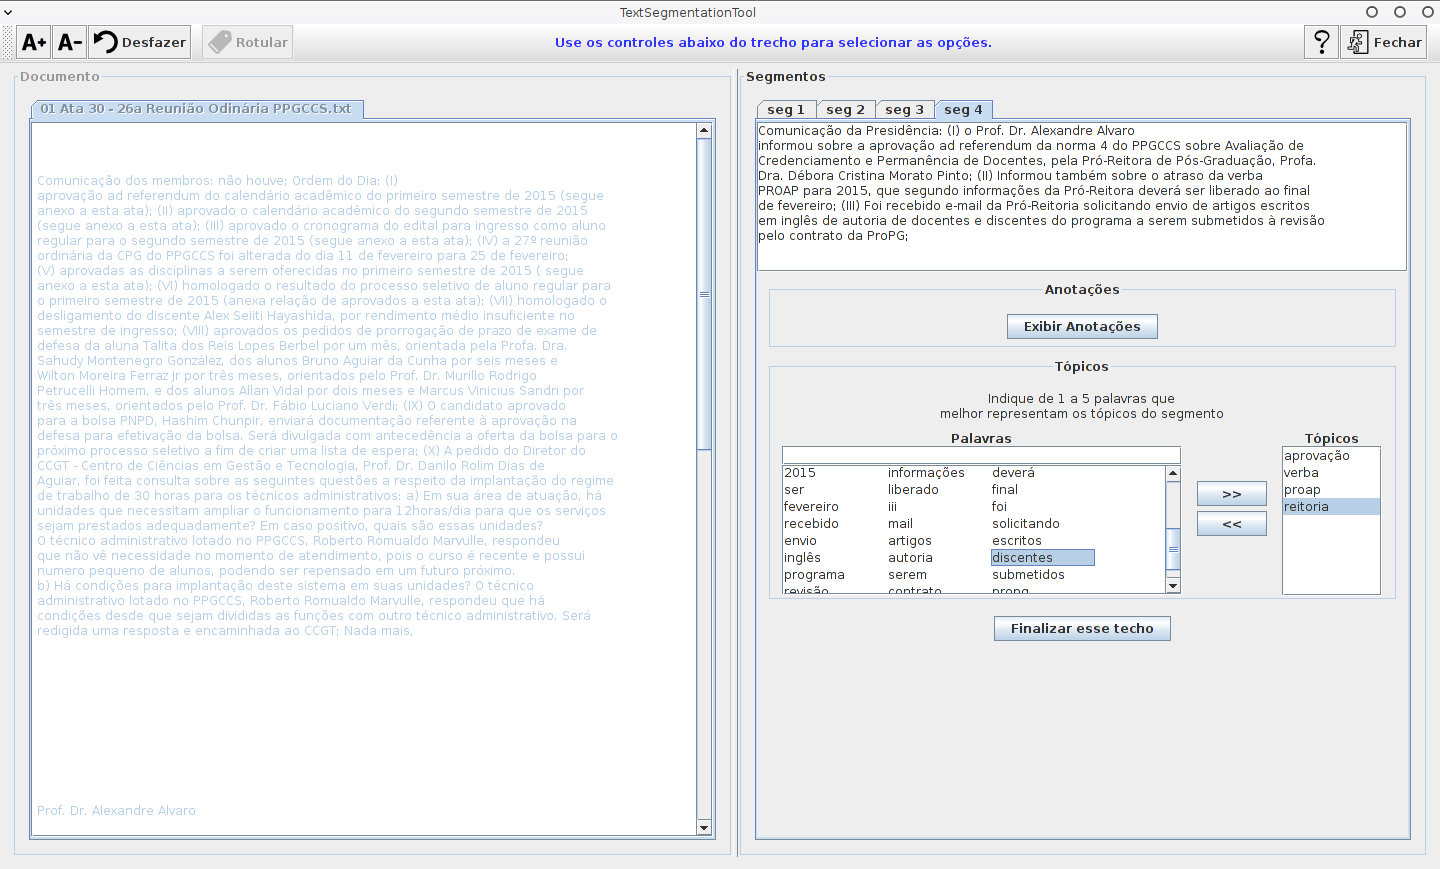
\includegraphics[width=1\textwidth]{conteudo/capitulos/figs/interface-anotacoes.png}
	  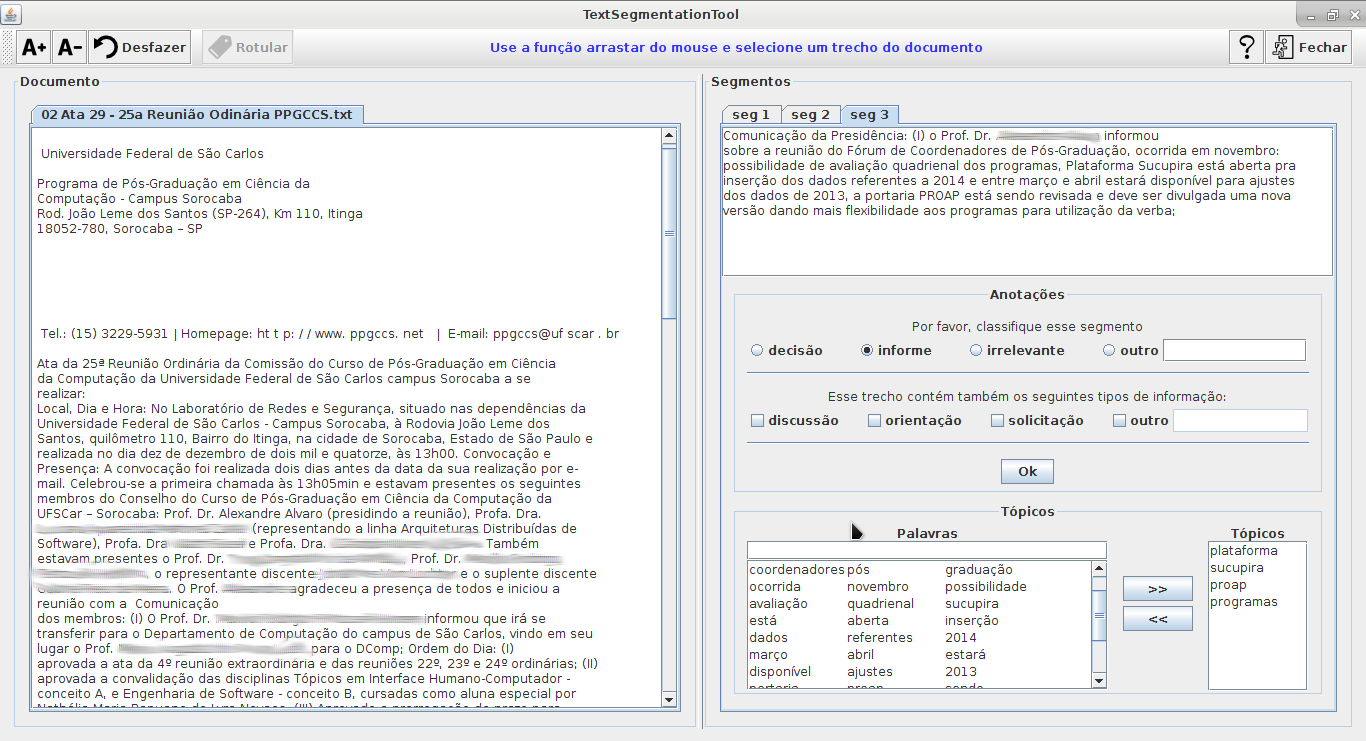
\includegraphics[width=1\textwidth]{conteudo/capitulos/figs/interface-TST.png}
	  \caption{Interface da ferramenta utilizada para anotações onde o texto a ser segmentado é exibido no painel a esquerda e os controles para anotação estão disponíveis a direita.}
	  \label{fig:interfaceanotacoes}
  \end{figure}



% -- 4 - Especificar o procedimento de anotação
O procedimento de anotação deu-se remotamente. Os anotadores receberam por e-mail o acesso ao \textit{software} e individualmente realizaram as anotações. A tarefa de segmentar e rotular manualmente demandou em torno de 4 a 6 horas de atenção dos anotadores. Em razão desse esforço, o \textit{software} permitiu que a tarefa fosse pausada e reiniciada sempre que houvesse necessidade, sem prejuízos ao trabalho.

O \textit{software} foi desenhado para padronizar o trabalho e otimizar o tempo dos anotadores. Ao mesmo tempo, dava dava liberdade para segmentar o texto após qualquer character do texto. Um segmento sempre deve terminar com um sentença completa, uma vez que as sentenças são a menor unidade de informação para os segmentadores, conforme explicado na seção~\ref{sec:aplicacao-sistema} e Algoritmo~\ref{alg:identificacaofinaisdesent}. Como previsto, houve casos onde o anotador omitiu ou adicionou characteres e palavras (quase sempre ocasionado por imprecisão durante a seleção do texto). Para garantir que todo segmento termine com uma sentença completa, aqueles que apresentavam sentenças incompletas tiveram seu incio ou final movidos para se adequar à saída dos algoritmos de segmentação. Após o processo, 12 atas foram segmentadas manualmente por 9 anotadores, gerando um conjunto de 108 anotações. Na Tabela~\ref{tab:ataseanotacoes}, é mostrado para cada ata a quantidade de sentenças do documento original e de segmentos identificados por cada anotador.



\begin{table}[!h]
	\centering
	\begin{tabular}{|l|c|c|c|c|c|c|c|c|c|c|c|c|c|} \hline
		\textbf{Ata} & \textbf{\#Sent.}  & 
		\textbf{A1}  & 
		\textbf{A2}  & 
		\textbf{A3}  & 
		\textbf{A4}  & 
		\textbf{A5}  & 
		\textbf{A6}  & 
		\textbf{A7}  & 
		\textbf{A8}  & 
		\textbf{A9} 
		\\	\hline
% 		              A1   A2   A3  A4    A5   A6   A7   A8   A9   
		Ata 1  & 25 & 7  & 4  & 11 & 6  & 16 & 8  & 8  & 15 & 16 \\ \hline 
		Ata 2  & 17 & 4  & 4  & 8  & 6  & 11 & 6  & 6  & 15 & 14 \\ \hline 
		Ata 3  & 26 & 6  & 6  & 8  & 4  & 15 & 9  & 10 & 18 & 14 \\ \hline 
		Ata 4  & 26 & 5  & 5  & 10 & 6  & 14 & 17 & 7  & 11 & 12 \\ \hline 
		Ata 5  & 33 & 4  & 4  & 6  & 5  & 17 & 22 & 9  & 18 & 16 \\ \hline 
		Ata 6  & 11 & 3  & 4  & 6  & 4  & 9  & 9  & 4  & 7  &  5 \\ \hline 
		Ata 7  & 20 & 3  & 7  & 5  & 4  & 11 & 14 & 5  & 5  &  4 \\ \hline 
		Ata 8  & 35 & 4  & 8  & 3  & 8  & 12 & 17 & 5  & 11 &  9 \\ \hline 
		Ata 9  & 24 & 3  & 5  & 3  & 6  & 11 & 11 & 3  & 9  &  9 \\ \hline 
		Ata 10 & 50 & 4  & 5  & 4  & 7  & 31 & 29 & 5  & 9  &  8 \\ \hline 
		Ata 11 & 43 & 4  & 7  & 5  & 7  & 29 & 19 & 5  & 9  & 12 \\ \hline 
		Ata 12 & 56 & 3  & 10 & 4  & 16 & 33 & 25 & 4  & 13 & 11 \\ \hline 
		\textbf{Total} &
		\textbf{366} & 
		\textbf{50}&  
		\textbf{69} & 
		\textbf{73}&  
		\textbf{79}&  
		\textbf{209} & 
		\textbf{186}&  
		\textbf{71}&  
		\textbf{140}&  
		\textbf{130} 
		\\ \hline 

	\end{tabular}
	\caption{Descrição dos resultados obtidos com anotadores. Na segunda coluna \#Sent., é mostrada a quantidade de sentenças de cada ata. Nas colunas A1-A9 é mostrado as quantidades de segmentos informados pelos anotadores. 
	% As colunas K, P$_k$ e WD indicam respectivamente as médias de \textit{Kappa}, $P_k$ e \textit{WindowDiff}.
} 

	\label{tab:ataseanotacoes}
\end{table}





% Os arquivos gerados foram tratados para que os segmentos sempre terminem em uma sentença reconhecida pelo algoritmo, uma vez que as sentenças são a unidade mínima de informação nesse trabalho.
O \textit{corpus} anotado deve ser constituído a partir dos textos originais e da resultante das percepções dos anotadores a cerca do fenômeno a ser explicado. Assim, o texto de cada uma das 12 atas selecionadas será acrescido de informações geradas a partir dos dados coletados. Após o processo de anotação, a segmentação de referência foi criada utilizando o critério de maior concordância, como já relatado em outros trabalhos~\cite{Hearst1997, Cardoso2017, Kazantseva2012, Passonneau1997, Galley2003}. Assim, considerou-se que ocorre um limite entre segmentos quando a maioria dos anotadores (metade mais um) concordou que a mesma sentença é um final de segmento. Gerou-se então 12 documentos derivados das atas originais os quais constituem a segmentação de referência utilizada nesse trabalho.

Na Figura~\ref{fig:concordanciasegref} é mostrado um exemplo de criação de uma segmentação de referência por meio da concordância entre anotadores. As primeiras linhas representam segmentações fornecidas por anotadores e a última linha representa a segmentação resultante da concordância entre a maioria dos segmentadores e portanto mais confiável. 

  \begin{center}
	\begin{figure}[h!]

	% 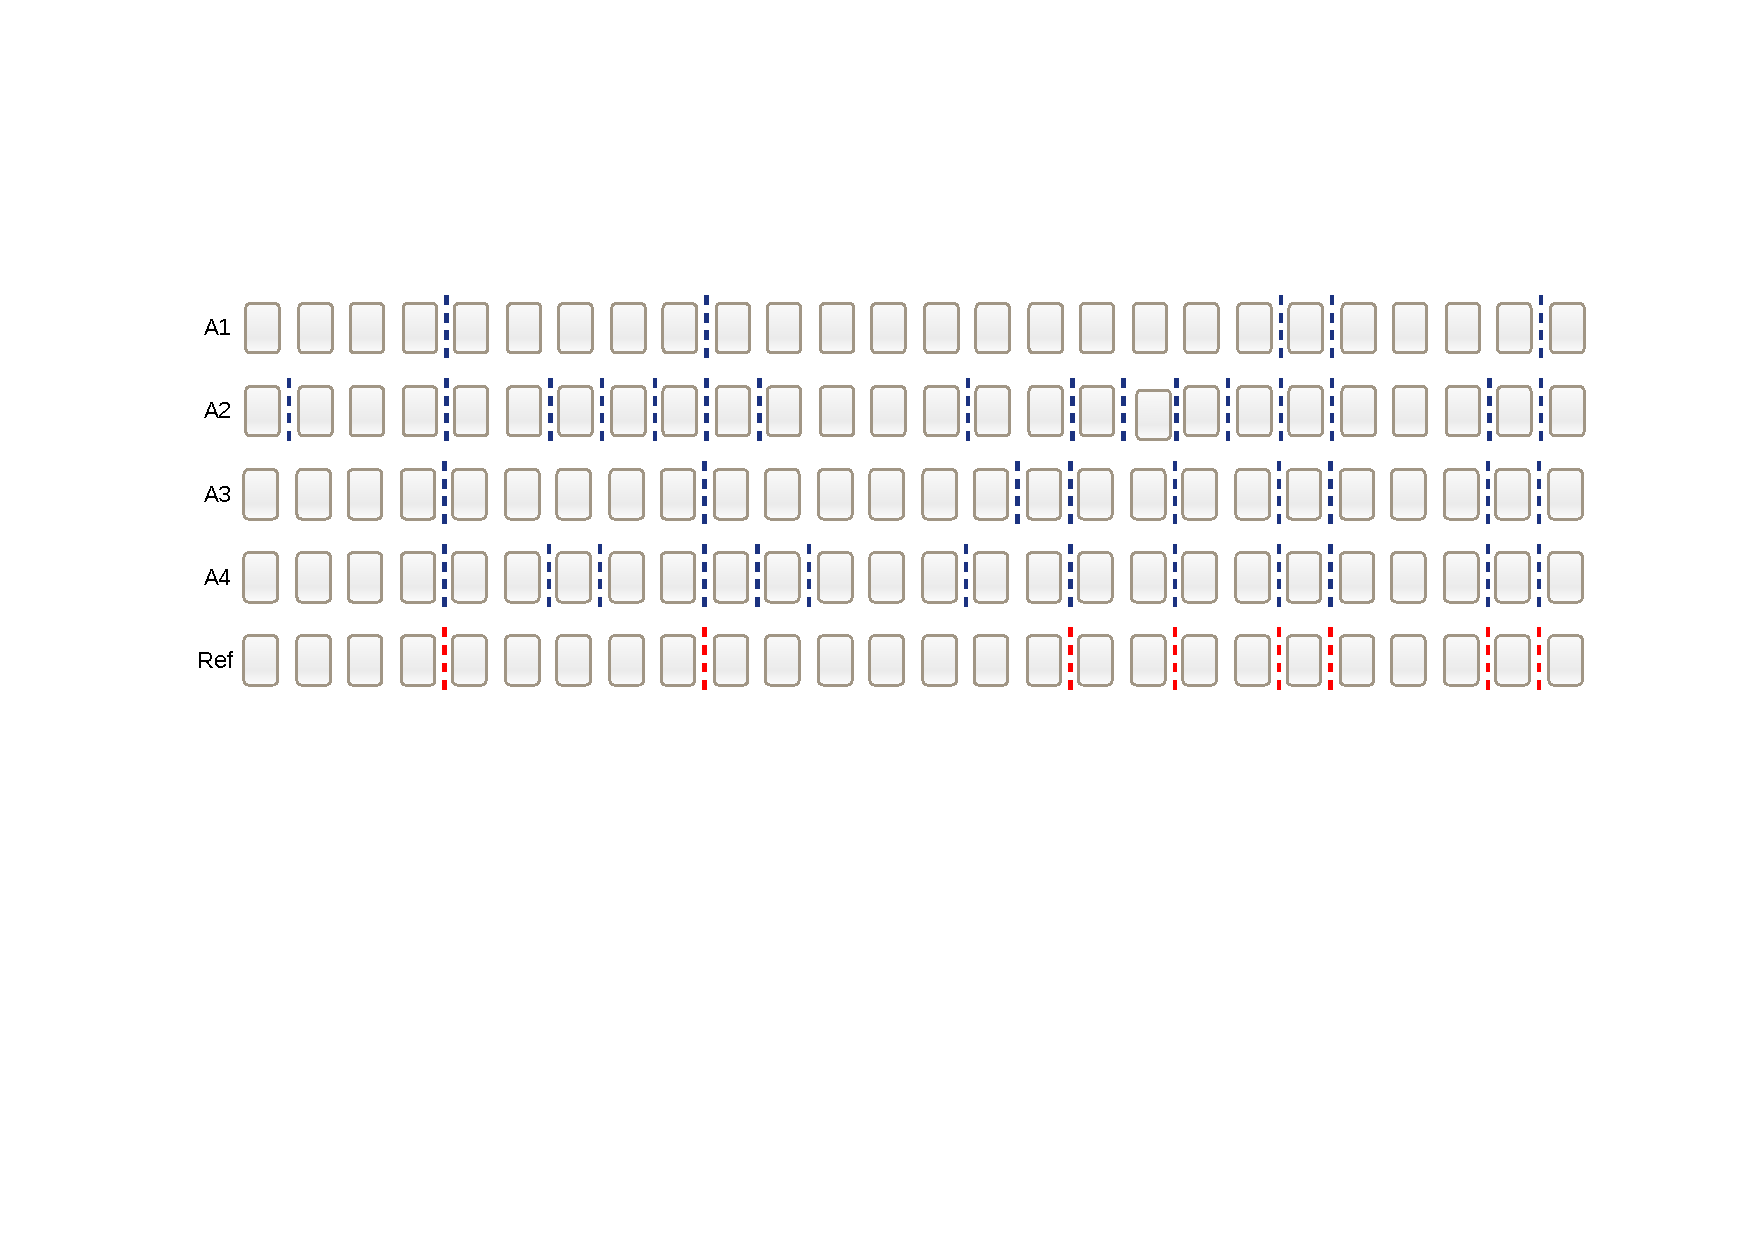
\includegraphics[trim={ 95 255 75 140 },clip,page=1,width=\textwidth]{conteudo/capitulos/figs/segmentacao-referencia.pdf}
	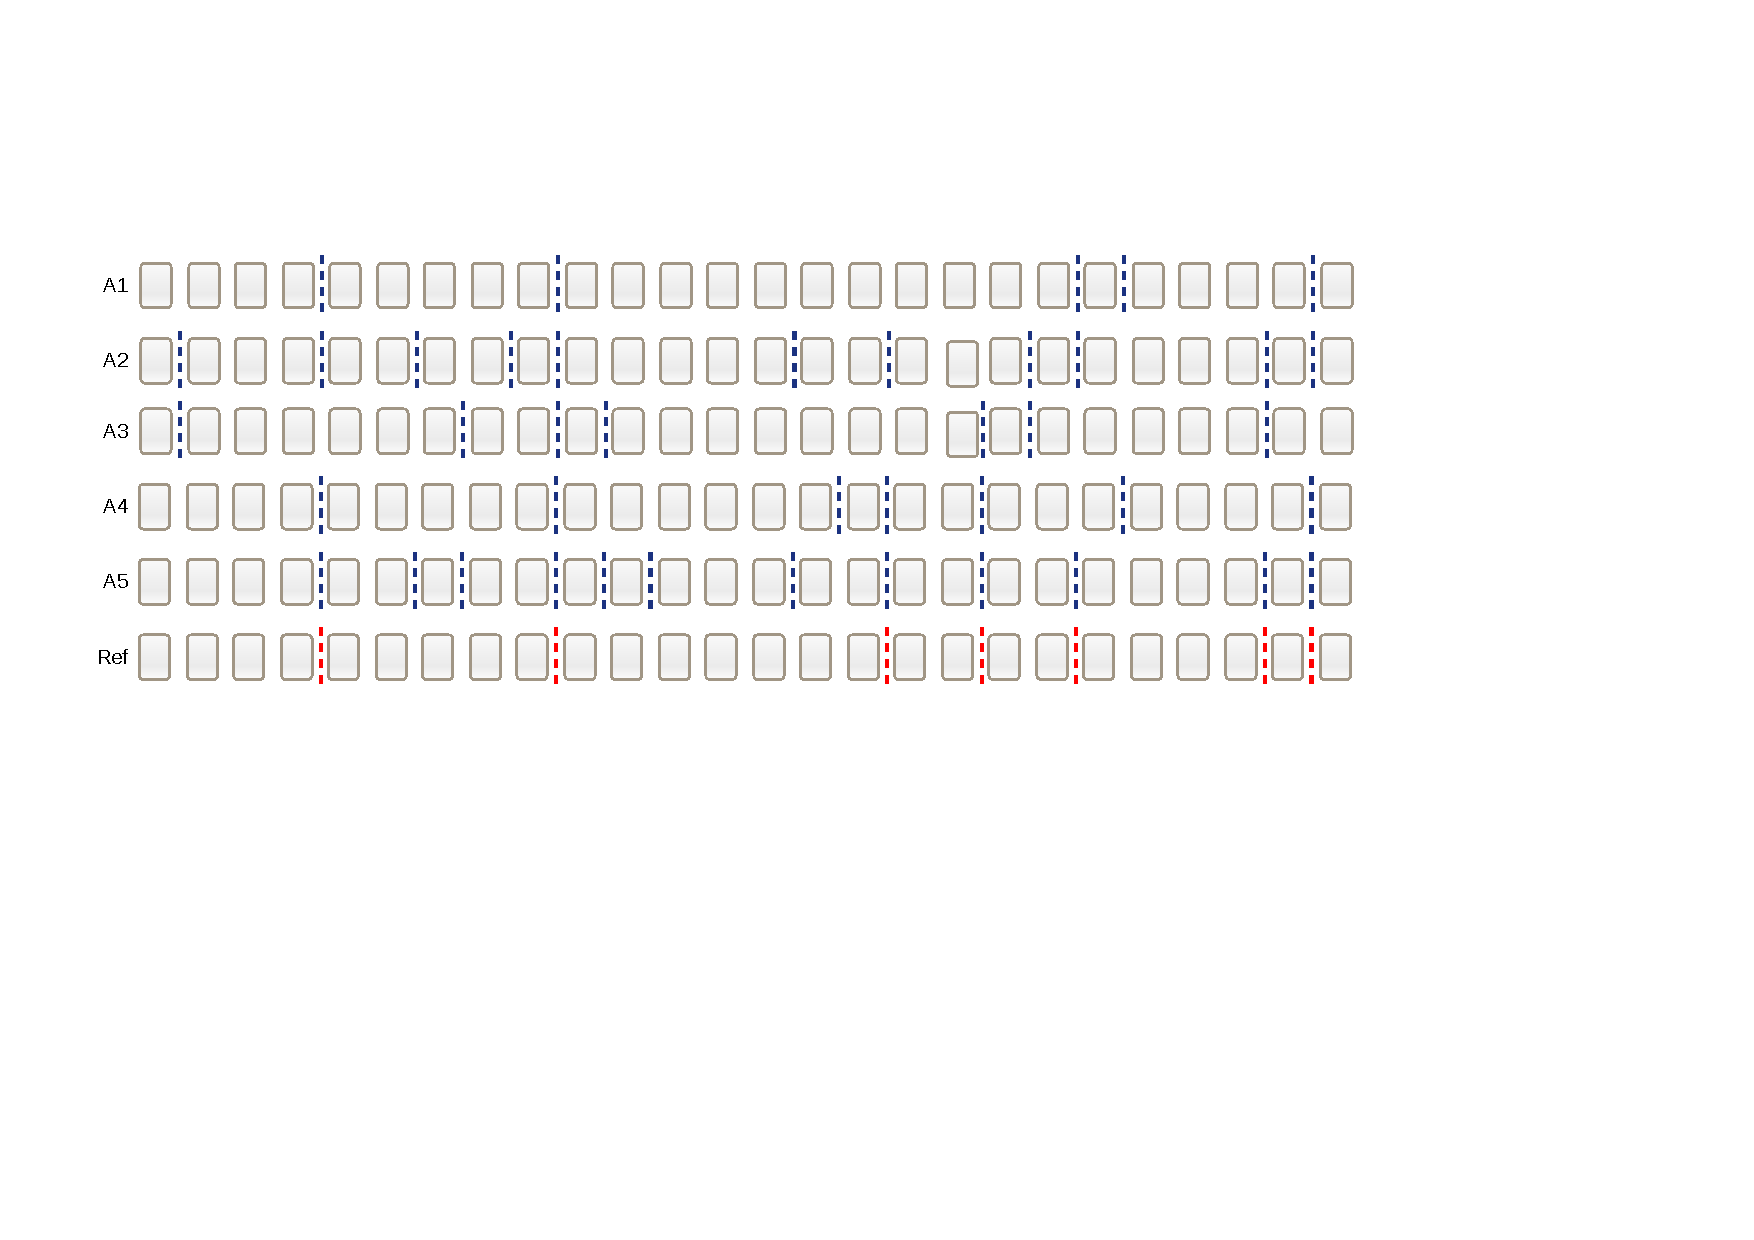
\includegraphics[trim={ 45 255 190 120 },clip,page=1,width=\textwidth]{conteudo/capitulos/figs/segmentacao-referencia-2.pdf}

	\caption{Exemplo uma segmentação de referência criada a partir da concordância entre segmentações manuais.}
	\label{fig:concordanciasegref}
	\end{figure}
\end{center}







% ----------------- Exemplo Segmentação de Referência ----------------------

Na Tabela~\ref{tab:segmentacaoreferencia} é mostrado um exemplo em que 6 dos 9 anotadores concordaram a respeito de um segmento. A tabela mostra quatro segmentos extraídos da segmentação de referência onde cada linha contém um segmento e os índices a esquerda indicam uma sentença. Junto à cada segmento é mostrada  a classe e descritores rotulados por um dos anotadores. Vale ressaltar que esses rótulos não foram utilizados no processo de segmentação e não têm nenhuma influência sobre a segmentação de referência. %Nesse trabalho, essas anotações são utilizadas na avaliação dos extratores de tópicos. --> não é

\begin{table}[!h]
	\centering 
\footnotesize
% \scriptsize
	\begin{tabular}{|p{0.2cm}p{14,5cm}|} \hline


$^{[7]}$&
(II) Encerrada a etapa de inscrição para o processo seletivo como aluno regular para o segundo semestre de 2015: foram quarenta e nove inscrições on-line e dezoito candidatos entregaram a documentação; 
\textit{<informe>} \textit{<processo;seletivo>}
\\ \hline


$^{[8]}$ &
(III) O Prof. Dr. AAA informou que a Pró-Reitora comunicou a oferta de mais uma bolsa pela cota da Pró-Reitoria, mas não havia aluno disponível para alocação da bolsa.\\
$^{[9]}$ &
(III) O Prof. Dr. AAA informou que a Pró-Reitora comunicou a oferta de mais uma bolsa pela cota da Pró-Reitoria, mas não havia aluno disponível para alocação da bolsa.\\
$^{[10]}$ &
O Prof. Dr. BBB informou que havia uma aluna interessada, mas não informada durante o processo de elaboração do ranking no início do semestre.\\
$^{[11]}$ &
Ficou decidido enviar e-mail aos docentes solicitando que comuniquem permanentemente interesse de alunos em bolsa pra atualização do ranking;
\textit{<informe>} \textit{<solicitação;bolsa;cota;ranking;alunos>}
\\ \hline


$^{[12]}$ &
(IV) Com a mudança do Prof. Dr. DDD para o campus de São Carlos, o Prof. Dr. BBB assume o posto de suplente da linha Teoria Aplicada à Computação na CPG;
\textit{<informe>} \textit{<mudança;suplente;teoria;aplicada;computação>}
\\ \hline

$^{[13]}$ &
	Comunicação dos membros: Não houve;
	\textit{<irrelevante>} 
\\ \hline



% $^{[14]}$ &
% Ordem do Dia: (I) Foram apresentadas regras para participação de membro externo em banca de defesa do mestrado.\\
% $^{[15]}$ &
% O Prof. Dr. Alexandre Alvaro comentou que está sendo pago aos participantes externos das bancas a diária pelo PROAP e o pró-labore pelo DComp, além do programa fornecer o transporte, que onera a verba PROAP.\\
% $^{[16]}$ &
% O Prof. Dr. Tiago Agostinho de Almeida sugeriu o seguinte cálculo para pagamento: se o participante vier de uma Instituição com distância até 220 km será feito o cálculo de R\$ 1,00 multiplicado pela quilometragem.\\
% $^{[17]}$ &
% Caso a distância seja superior a 220 km, será calculada a distância multiplicada por R\$ 0,60. O menor valor entre o custo do transporte e o pagamento de verba e pró-labore será utilizado para custear a vinda do participante;
% \\ \hline



% $^{[18]}$ &
% (II) Foi discutida a forma de convalidação de disciplinas cursadas como aluno regular anterior a três anos do reingresso do aluno.
% Foi decidido que fica a cargo da CPG decidir sobre as disciplinas que serão aproveitadas quando do reingresso do aluno;
% \\ \hline



% $^{[13]}$ &

	\end{tabular}
	\caption{Exemplo de segmentação de referência com rotulação de um anotador}
	\label{tab:segmentacaoreferencia}
\end{table}








  




% -- 6 - Escolher e aplicar medidas de avaliação
A qualidade da segmentação de referência está ligada principalmente a conformidade das anotações quanto a atribuição de final de segmento a cada sentença.
Para mensurar a concordância entre anotadores, a medida \textit{kappa (k)}~\cite{Carletta1996} é frequentemente utilizada~\cite{Gruenstein2007, Cardoso2017, Hearst1997}. Ela mostra como os anotadores compreendem os textos analisados e o nível de confiabilidade da segmentação de referência. Essa medida retorna um valor no intervalo de 0 até 1, onde 1 significa uma concordância perfeita e 0 que não houve concordância. 
% As medidas de similaridade entre segmentações também podem ser utilizadas para avaliar a qualidade da segmentação de referência. 
As medidas \textit{WindowDiff} e $P_k$ informam a probabilidade de duas sentenças escolhidas aleatoriamente estarem no mesmo segmento. Elas refletem a similaridade entre duas segmentações, assim também podem ser utilizadas para avaliar a concordância entre os anotadores. As formulações dessas medidas são abordadas em mais detalhes na Seção~\ref{subsec:medidas-segmentacao}.
%
%
Nesse trabalho calculou-se as medidas \textit{WindowDiff}, $P_k$ e \textit{Kappa} para cada par de anotação referente a cada ata, ou seja, para cada uma das 12 atas calculou-se a concordância entre os anotadores.  
A Tabela~\ref{tab:detalhesSegRef} contém, para cada ata, a quantidade de sentenças e a quantidade de segmentos identificadas pelos participantes e as médias de \textit{WindowDiff}, $P_k$ e \textit{Kappa}. Uma vez que P$_k$ e \textit{WindowDiff}, são medidas de dissimilaridade, são reportados os seus complementos.
% Uma vez que P$_k$ e WD, indicam melhores valores próximos a 0 e 1 como dissimilarid 




% - maior granularidade é preferivel, pois evita omição de informação.




\begin{table}[!h]
	\centering
 \begin{tabular}{|c|c|c|c|c|}

\hline
\textbf{Referência}  & \textbf{\#Seg} & \textbf{\textit{Kappa}}  & \textbf{\textit{P}$_k$}                &  \textbf{\textit{WinDiff}}\\ 
	& & Média (des. pad.) & Média (des. pad.)&Média (des. pad.) \\ \hline
Ref. 01     & 15    & 0,344  (0,190) & 0,433  (0,170) & 0,631  (0,409) \\ \hline
Ref. 02     & 13    & 0,266  (0,246) & 0,439  (0,190) & 0,565  (0,379) \\ \hline
Ref. 03     & 15    & 0,328  (0,183) & 0,442  (0,165) & 0,590  (0,353) \\ \hline
Ref. 04     & 15    & 0,364  (0,241) & 0,364  (0,161) & 0,562  (0,377) \\ \hline
Ref. 05     & 19    & 0,315  (0,217) & 0,458  (0,223) & 0,889  (0,640) \\ \hline
Ref. 06     & 9     & 0,314  (0,218) & 0,404  (0,163) & 0,463  (0,266) \\ \hline
Ref. 07     & 8     & 0,235  (0,208) & 0,343  (0,192) & 0,507  (0,401) \\ \hline
Ref. 08     & 12    & 0,211  (0,225) & 0,421  (0,186) & 0,629  (0,479) \\ \hline
Ref. 09     & 12    & 0,234  (0,258) & 0,472  (0,203) & 0,660  (0,427) \\ \hline
Ref. 10     & 13    & 0,170  (0,206) & 0,428  (0,227) & 0,937  (1,050) \\ \hline
Ref. 11     & 12    & 0,209  (0,236) & 0,368  (0,203) & 0,704  (0,654) \\ \hline
Ref. 12     & 21    & 0,222  (0,195) & 0,452  (0,200) & 0,113  (1,202) \\ \hline
\textbf{Total}      & \textbf{13.666} & \textbf{0,267}  \textbf{(0,218)} & \textbf{0,418}  \textbf{(0,190)} & \textbf{0,604}  \textbf{(0,553)} \\ \hline
\end{tabular}
\caption{Medidas de concordância entre os anotadores sobre cada ata segmentada manualmente.}
\label{tab:detalhesSegRef}
\end{table}




Os valores de \textit{Kappa} reforçam que a tarefa de segmentação é bastante subjetiva e indicam que, nesse contexto, a segmentação de referência resultante é pouco confiável, visto os baixos valores de concordância entre os anotadores. 
Embora~\cite{Carletta1996} afirme que valores de $k~>~0,8$ indicam que os dados são confiáveis, visto a subjetividade da tarefa de segmentação textual, medidas menores podem ser aceitáveis, como reportado em~\cite{Hearst1997} que obteve $k~=~0,64$ e~\cite{Cardoso2017}, que obteve $k~=~0,56$. Além dos baixos valores para as medidas nota-se também que os anotadores divergem na quantidade de segmentos, o que sugere que diferentes anotadores tem percepções distintas quanto a granularidade de assuntos, ou seja, trechos com pequenas mudanças de assunto são entendidas como segmentos diferentes por alguns anotadores, enquanto outros entendem como pertencentes ao mesmo assunto.

% -- 7 - disponibilizar e manter o produto
Após a coleta dos dados das anotações e construção da segmentação de referência, o \textit{corpus} anotado serviu de como base para avaliação dos segmentadores bem como aspectos da configuração e avaliação dos extratores de tópicos no Capítulo~\ref{cap-extratores}. O produto resultante do processo de anotação, constituído por segmentos de atas anotados está disponibilizado\footnote{Acessível em  \url{https://github.com/ovidio-francisco/UFSCar/}} para outros trabalhos voltados a esse domínio. 








\section{Configuração Experimental}
\label{subsec:configuracaoexperimental}

  
Para avaliação objetiva dos algoritmos, faz-se necessário encontrar os valores de parâmetros que melhor configuram cada algoritmo.
% -> Parâmetros do TT
O \textit{TextTiling} permite ajustar dois parâmetros, sendo o tamanho da janela e o passo. Por meio de testes empíricos escolheu-se os valores os valores 20, 40 e 60 para o tamanho da janela e 3, 6, 9 e 12 para o passo, gerando ao final 20 configurações, resultantes da combinação desses dois parâmetros.
%

% -> Parâmetros do C99
O \textit{C99} possui três parâmetros: 
a quantidade de segmentos desejados, 
o tamanho do quadro utilizado para gerar a matriz de ranking e
a representação dos atributos das sentenças.
Para o primeiro parâmetro, referente à quantidade segmentos desejados, uma vez que não se conhece o número ideal de segmentos, configurou-se a quantidade de segmentos com base em uma proporção dos candidatos a limite. Para isso atribuiu-se os valores {0,2; 0,4; 0,6; 0,8}. 
Para o segundo parâmetro, referente ao tamanho do quadro utilizado para gerar a matriz de ranking, atribuiu-se os valores 9 e 11, sendo 11 o valor padrão apresentado pelo autor. 
O algoritmo permite ainda indicar se as sentenças serão representadas por vetores contendo a frequência ou o peso de cada termo. Ambas as representações foram utilizadas. Considerando todos os parâmetros, foram geradas 16 configurações para o algoritmo \textit{C99}.

Os algoritmos tradicionais baseados em coesão léxica como o \textit{TextTiling} e \textit{C99} são fortemente afetados pela distribuição das palavras no texto, pois a maioria das medidas de similaridade, como a cosseno utilizada nesses algoritmos, baseiam-se na frequência das palavras. Para esses, a remoção de termos menos significativos na etapa de pré-processamento pode influenciar o desempenho. Para outras abordagens como \textit{MinCutSeg} e \textit{BayesSeg}, usou-se as configurações fornecidas por~\cite{Eis2008}, onde essas técnicas foram utilizadas como \textit{base line}. Para o \textit{TextSeg} é requerido apenas a configuração da quantidade de segmentos a serem identificados.
Há ainda outras estratégias passíveis de aplicação, como a utilização de fontes externas, por exemplo \textit{thesaurus} e palavras pista, como discutido em \cite{Naili2016, Gutierrez2016, Ferret2009}. Nesse trabalho, essas estratégias não são utilizadas para manter uma abordagem não supervisionada e independente de domínio. 

% Inicialmente, 
Calculou-se as medidas configurando cada algoritmo
% conforme mostrado na Subseção~\ref{subsec:configuracaoexperimental} e, 
a fim de conhecer o impacto do pré-processamento nos algoritmos. 
% \textit{TextTiling} e \textit{C99}
Esses foram testados em duas etapas: com o texto integral, e com o texto pré-processado em que elementos menos significativos foram removidos, conforme mencionado na Seção~\ref{sec:modulo-preparacao}.  


\section{Critérios de Avaliação}

% -> Definição do que é um bom algoritmo de segmentação
Para fins de avaliação desse trabalho, um bom método de segmentação é aquele cujo resultado melhor se aproxima da segmentação de referência, sem a obrigatoriedade de estar perfeitamente alinhado com tal. Ou seja, visto o contexto das atas de reunião, e a subjetividade da tarefa, não é necessário que os limites entre os segmentos (real e hipótese) sejam idênticos, mas que se assemelhem em localização e quantidade.

As segmentações obtidas com os algoritmos foram comparadas com a segmentação de referência obtida e calculou-se as medidas mais aplicadas à segmentação textual, $P_k$ e \textit{WindowDiff}. Além dessas, computou-se também as medidas tradicionais Acurácia e $F^1$ para análises que consideram a exatidão dessas técnicas.
% comparação com outros trabalhos que as utilizam.
%
% O teste de Friedman foi utilizado para gerar um ranking das melhores configurações para cada medida calculada. Com isso, foi possível descobrir quais valores otimizam um algoritmo para cada medida, considerando seus parâmetros e a influência do pré-processamento. 
% Como já mencionado, os algoritmos \textit{MinCutSeg} e \textit{BayesSeg} aplicou-se a etapa de pré-processamento e foram testados com as configurações apresentadas por~\cite{Eis2008}. 



\section{Resultados}

Obteve-se por meio dos testes apresentados as melhores configurações para as principais medidas de avaliação de segmentadores. Com essas configurações calculou-se a média de cada medida considerando o conjunto de documentos. Os algoritmos foram executados com as configurações apresentadas e discutidos mais adiante nessa seção.

A seguir são apresentados os resultados obtidos com os algoritmos baseados em coesão léxica 
% (\textit{TextTiling} e \textit{C99}), 
considerando seus principais parâmetros e a aplicação do pré-processamento. Em seguida, são apresentados os resultados da avaliação geral de todos os algoritmos abordados nesse trabalho.
Na Tabela~\ref{tab:resultados-tt-pp} são apresentadas, as médias das medidas de desempenho obtidas com o \textit{TextTiling} bem como as configurações utilizadas.


	
\begin{table}[!h]
\center
\textbf{TextTiling} \\ 
	\begin{tabular}{|c|c||c|c|c|c|c||c|c|c|c|c|}
\hline 
\multirow{2}{*}{Step} & \multirow{2}{*}{Win Size}
  & \multicolumn{5}{c||}{Com texto pré-processado} & \multicolumn{5}{|c|}{Com texto integral}\\\cline{3-12} 
&& $WinDiff$ & $P_k$ & Acurácia & $F^1$ & \#Segs &  $WinDiff$ & $P_k$ & Acurácia & $F^1$ & \#Segs\\ \hline 
 \multirow{6}{*}{20} 
  & 30 & 0.513 & 0.490 & 0.538 & 0.334  & 8.500                 & 0,461 & 0,444 & 0,581 & \cellcolor{gray!20} \textbf{0,411} & 8,833  \\ \cline{2-12} 
  & 35 & 0.509 & 0.492 & 0.540 & 0.350  & 8.583                 & 0,462 & 0,443 & 0,582 & 0,401 & 8,750  \\  \cline{2-12}
  & 40 & 0.517 & 0.495 & 0.532 & 0.342  & 8.583                 & 0,485 & 0,466 & 0,562 & 0,378 & 8,250  \\  \cline{2-12}
  & 45 & 0.496 & 0.477 & 0.555 & 0.347  & 7.667                 & 0,480 & 0,458 & 0,572 & 0,369 & 8,250  \\  \cline{2-12}
  & 50 & 0.481 & 0.465 & 0.569 & \cellcolor{gray!20} \textbf{0.390} & 8.750  & 0,523 & 0,503 & 0,528 & 0,327 & 8,417  \\  \cline{2-12}
  & 55 & 0.512 & 0.493 & 0.542 & 0.337  & 8.250  & 0,491 & 0,474 & 0,549 & 0,331 & 8,250  \\ \hline      
 \multirow{6}{*}{30} 
  & 30 & 0.511 & 0.494 & 0.538 & 0.284  & 6.667                & 0,509 & 0,488 & 0,536 & 0,286 & 6,917  \\ \cline{2-12}    
  & 35 & 0.517 & 0.500 & 0.536 & 0.285  & 6.583                & 0,500 & 0,479 & 0,551 & 0,318 & 7,167  \\ \cline{2-12}         
  & 40 & 0.512 & 0.491 & 0.543 & 0.299  & 6.750                & 0,468 & 0,451 & 0,576 & 0,348 & 6,750  \\ \cline{2-12} 
  & 45 & 0.502 & 0.483 & 0.555 & 0.320  & 6.917                & \cellcolor{gray!20} \textbf{0,450} & \cellcolor{gray!20} \textbf{0,435} & \cellcolor{gray!20} \textbf{0,596} & 0,373 & 6,417  \\  \cline{2-12} 
  & 50 & 0.510 & 0.493 & 0.539 & 0.313  & 7.333                & 0,493 & 0,478 & 0,543 & 0,307 & 6,417  \\ \cline{2-12}                
  & 55 & 0.498 & 0.480 & 0.543 & 0.328  & 7.250                & 0,481 & 0,463 & 0,558 & 0,346 & 7,083  \\ \hline     
 \multirow{6}{*}{40} 
  & 30 & 0.493 & 0.477 & 0.555 & 0.248  & 4.917                & 0,475 & 0,460 & 0,566 & 0,306 & 5,833  \\ \cline{2-12} 
  & 35 & 0.482 & 0.465 & 0.558 & 0.267  & 5.417                & 0,501 & 0,482 & 0,542 & 0,268 & 6,083  \\ \cline{2-12} 
  & 40 & 0.476 & 0.459 & 0.565 & 0.275  & 5.500                & 0,499 & 0,478 & 0,548 & 0,293 & 6,083  \\ \cline{2-12} 
  & 45 & 0.501 & 0.482 & 0.549 & 0.260  & 5.333                & 0,488 & 0,471 & 0,551 & 0,275 & 5,500  \\ \cline{2-12} 
  & 50 & 0.498 & 0.481 & 0.551 & 0.266  & 5.333                & 0,495 & 0,474 & 0,552 & 0,280 & 5,833  \\ \cline{2-12} 
  & 55 & 0.505 & 0.487 & 0.544 & 0.243  & 5.083                & 0,476 & 0,453 & 0,567 & 0,310 & 6,083  \\ \hline      
 \multirow{6}{*}{50} 
 & 30 & \cellcolor{gray!20} \textbf{0.474} & \cellcolor{gray!20} \textbf{0.455} & \cellcolor{gray!20} \textbf{0.579} & 0.295 & 4.917 & 0,492 & 0,473 & 0,557 & 0,274 & 5,167  \\ \cline{2-12}
  & 35 & 0.528 & 0.511 & 0.531 & 0.202  & 4.583                & 0,504 & 0,484 & 0,549 & 0,268 & 5,583  \\ \cline{2-12} 
  & 40 & 0.501 & 0.488 & 0.539 & 0.234  & 5.000                & 0,501 & 0,481 & 0,556 & 0,278 & 5,417  \\ \cline{2-12} 
  & 45 & 0.489 & 0.476 & 0.558 & 0.275  & 5.167                & 0,508 & 0,484 & 0,549 & 0,264 & 5,500  \\ \cline{2-12} 
  & 50 & 0.498 & 0.483 & 0.545 & 0.304  & 6.083                & 0,513 & 0,491 & 0,536 & 0,253 & 5,417  \\ \cline{2-12} 
  & 55 & 0.490 & 0.470 & 0.556 & 0.303  & 5.583                & 0,509 & 0,487 & 0,543 & 0,276 & 5,833  \\ \hline      
 \multirow{6}{*}{60}                           
  & 30 & 0.499 & 0.486 & 0.557 & 0.234  & 4.417                & 0,481 & 0,462 & 0,564 & 0,267 & 4,917  \\ \cline{2-12} 
  & 35 & 0.509 & 0.494 & 0.537 & 0.243  & 5.000                & 0,503 & 0,483 & 0,549 & 0,250 & 5,083  \\ \cline{2-12} 
  & 40 & 0.501 & 0.486 & 0.545 & 0.182  & 3.833                & 0,497 & 0,481 & 0,554 & 0,242 & 4,750  \\ \cline{2-12} 
  & 45 & 0.493 & 0.478 & 0.558 & 0.227  & 4.167                & 0,465 & 0,448 & 0,577 & 0,271 & 4,500  \\ \cline{2-12} 
  & 50 & 0.495 & 0.478 & 0.562 & 0.225  & 4.083                & 0,478 & 0,459 & 0,569 & 0,250 & 4,333  \\ \cline{2-12} 
  & 55 & 0.500 & 0.485 & 0.550 & 0.198  & 4.000                & 0,474 & 0,457 & 0,568 & 0,269 & 5,000  \\ \hline      

 \end{tabular}  
\caption{Resultados do TextTiling considerando o pré-processamento.}
\end{table} 

  



Observou-se que o \textit{TextTiling} produz resultados muito similares em relação ao texto pré-processado e o texto integral. A quantidade de segmentos obtidos é influenciada por \textbf{Step} e \textbf{WS} (\textit{Win Size}), em que menores valores desses parâmetros tendem a produzir mais segmentos, que por consequência também refletem em melhores valores para $F^1$, pois que essa medida é baseada na precisão, a qual é fortemente afetada por falsos positivos. Os melhores valores de \textit{WinDiff} e $P_k$ coincidem nas mesmas configurações que também apresentam resultados mais acurados. A relação entre essas medidas é discutida mais adiante nessa seção.

% visto que a primeira é baseada na segunda 
% Nota-se também que os menores valores para Step e Win Size 



\begin{table}[!h]
	\center
	\textbf{C99}  \\
	\begin{tabular}{|c|c|c||c|c|c|c||c|c|c|c||c|} 
\hline 
\multirow{2}{*}{W} & \multirow{2}{*}{RS} & \multirow{2}{*}{SR} & \multicolumn{4}{c||}{Com texto pré-processado} & \multicolumn{4}{c||}{Com texto integral}& \multirow{2}{*}{\#Segs} \\\cline{4-11}

&& & $WinDiff$ & $P_k$ & Acurácia & $F^1$ & $WinDiff$ & $P_k$ & Acurácia & $F^1$ & \\ \hline 
 \multirow{18}{*}{true} & \multirow{6}{*}{3} 
	 & 0,20    & 0,481 & 0,463 & 0,574 & 0,324         &     0,463 &  0,445 & 0,581 & 0,339 & 6,083                \\ \cline{3-12}
	&& 0,30    & 0,457 & 0,437 & 0,596 & 0,447         &     \cellcolor{gray!20} \textbf{0,434} & \cellcolor{gray!20} \textbf{0,407} & 0,607 & 0,457 & 9,250  \\\cline{3-12} 
	&& 0,40    & 0,450 & 0,425 & 0,602 & 0,513         &     0,452 &  0,422 & 0,604 & 0,515 & 12,083              \\ \cline{3-12}                                            
	&& 0,50    & \cellcolor{gray!20} \textbf{0,435} & \cellcolor{gray!20} \textbf{0,395} & \cellcolor{gray!20} \textbf{0,629} & 0,594  &     0,499 &  0,458 & 0,577 & 0,539 & 15,500              \\ \cline{3-12}
	&& 0,60    & 0,489 & 0,437 & 0,592 & 0,591 & 18,417                                &     0,487 &  0,440 & 0,592 & 0,591               \\ \cline{3-12}                 
	&& 0,70    & 0,482 & 0,420 & 0,602 & \cellcolor{gray!20} \textbf{0,632} &    0,485 &  0,431 & 0,602 & \cellcolor{gray!20} \textbf{0,633} & 21,417 \\ \cline{2-12} 
 & \multirow{6}{*}{5} 
	  & 0,20    & 0,488 & 0,469 & 0,565 & 0,313         &     0,454 &  0,437 & 0,583 & 0,338 & 6,083               \\ \cline{3-12}                  
	 && 0,30    & 0,476 & 0,458 & 0,571 & 0,426         &     0,454 &  0,434 & 0,595 & 0,446 & 9,250               \\ \cline{3-12}                  
	 && 0,40    & 0,476 & 0,452 & 0,578 & 0,487         &     0,475 &  0,443 & 0,590 & 0,497 & 12,083              \\ \cline{3-12}                  
	 && 0,50    & 0,463 & 0,425 & 0,605 & 0,566         &     0,460 &  0,421 & \cellcolor{gray!20} \textbf{0,609} & 0,571 & 15,500  \\ \cline{3-12} 
	 && 0,60    & 0,464 & 0,415 & 0,610 & 0,604         &     0,491 &  0,442 & 0,591 & 0,588 & 18,417              \\ \cline{3-12}                  
	 && 0,70    & 0,504 & 0,435 & 0,589 & 0,619         &     0,525 &  0,449 & 0,576 & 0,609 & 21,417              \\ \cline{2-12}                  
 & \multirow{6}{*}{7}                                                                                                                               
	  & 0,20    & 0,478 & 0,459 & 0,574 & 0,328         &     0,491 &  0,474 & 0,555 & 0,293 & 6,083               \\ \cline{3-12}                  
	 && 0,30    & 0,481 & 0,462 & 0,570 & 0,418         &     0,486 &  0,469 & 0,565 & 0,395 & 9,250               \\ \cline{3-12}                  
	 && 0,40    & 0,478 & 0,452 & 0,577 & 0,482         &     0,502 &  0,472 & 0,561 & 0,453 & 12,083              \\ \cline{3-12}                  
	 && 0,50    & 0,471 & 0,427 & 0,604 & 0,563         &     0,460 &  0,421 & 0,604 & 0,561 & 15,500              \\ \cline{3-12}                  
	 && 0,60    & 0,480 & 0,429 & 0,599 & 0,594         &     0,486 &  0,433 & 0,591 & 0,585 & 18,417              \\ \cline{3-12}                  
	 && 0,70    & 0,516 & 0,444 & 0,579 & 0,611         &     0,547 &  0,470 & 0,551 & 0,586 & 21,417              \\ \hline                       
\multirow{18}{*}{false} & \multirow{6}{*}{3} 
	  & 0,20    & 0,469 & 0,453 & 0,579 & 0,335         &     0,448 &  0,427 & 0,596 & 0,362 & 6,083               \\ \cline{3-12}  
	 && 0,30    & 0,441 & 0,421 & 0,608 & 0,463         &     0,454 &  0,426 & 0,594 & 0,445 & 9,250               \\ \cline{3-12}  
	 && 0,40    & 0,467 & 0,439 & 0,591 & 0,493         &     0,490 &  0,455 & 0,568 & 0,469 & 12,083              \\ \cline{3-12}  
	 && 0,50    & 0,483 & 0,442 & 0,593 & 0,554         &     0,529 &  0,481 & 0,543 & 0,503 & 15,500              \\ \cline{3-12}  
	 && 0,60    & 0,500 & 0,442 & 0,589 & 0,587         &     0,554 &  0,499 & 0,528 & 0,535 & 18,417              \\ \cline{3-12}  
	 && 0,70    & 0,492 & 0,423 & 0,602 & 0,632         &     0,565 &  0,496 & 0,526 & 0,570 & 21,417              \\ \cline{2-12}  
& \multirow{6}{*}{5}                                                                                                                
	  & 0,20    & 0,495 & 0,476 & 0,555 & 0,300         &     0,498 &  0,479 & 0,545 & 0,277 & 6,083               \\ \cline{3-12}  
	 && 0,30    & 0,503 & 0,485 & 0,549 & 0,386         &     0,505 &  0,482 & 0,540 & 0,369 & 9,250               \\ \cline{3-12}  
	 && 0,40    & 0,496 & 0,477 & 0,564 & 0,466         &     0,536 &  0,504 & 0,520 & 0,407 & 12,083              \\ \cline{3-12}  
	 && 0,50    & 0,488 & 0,452 & 0,574 & 0,533         &     0,540 &  0,490 & 0,529 & 0,485 & 15,500              \\ \cline{3-12}  
	 && 0,60    & 0,484 & 0,434 & 0,594 & 0,592         &     0,529 &  0,469 & 0,545 & 0,543 & 18,417              \\ \cline{3-12}  
	 && 0,70    & 0,522 & 0,451 & 0,574 & 0,609         &     0,542 &  0,464 & 0,549 & 0,584 & 21,417              \\ \cline{2-12}  
& \multirow{6}{*}{7}                                                                                                                
	  & 0,20    & 0,489 & 0,471 & 0,560 & 0,307         &     0,512 &  0,495 & 0,534 & 0,250 & 6,083               \\ \cline{3-12}  
	 && 0,30    & 0,498 & 0,479 & 0,554 & 0,394         &     0,527 &  0,506 & 0,522 & 0,336 & 9,250               \\ \cline{3-12}  
	 && 0,40    & 0,500 & 0,475 & 0,561 & 0,462         &     0,530 &  0,494 & 0,535 & 0,420 & 12,083              \\ \cline{3-12}  
	 && 0,50    & 0,479 & 0,441 & 0,592 & 0,551         &     0,503 &  0,454 & 0,571 & 0,523 & 15,500              \\ \cline{3-12}  
	 && 0,60    & 0,493 & 0,439 & 0,585 & 0,586         &     0,511 &  0,453 & 0,565 & 0,562 & 18,417              \\ \cline{3-12}  
	 && 0,70    & 0,506 & 0,430 & 0,590 & 0,621         &     0,559 &  0,476 & 0,535 & 0,572 & 21,417              \\ \hline      
 \end{tabular}  
\caption{Resultados do TextTiling considerando o pré-processamento.}
\end{table} 
  


Na Tabela~\ref{tab:resultadosc99} são apresentadas, as médias obtidas com o \textit{C99} bem como as configurações utilizadas, onde \textbf{SR} (\textit{Segment Rate}) é a proporção de segmentos em relação a quantidade de candidatos, \textbf{RS} (\textit{Ranking Size}) é o tamanho do quadro utilizado para criar a matriz de \textit{rankings} e \textbf{W} indica se as sentenças são representadas por vetores contendo a frequência dos termos ou um peso que representa sua importância no documento. % como TF*IDF que seria a frequencia do termo no elemento (sentença ou parágrafo) * a frequecia invertida do termo no documento. 
% indica se os segmentos são representados por vetores contendo a frequência ou um peso das palavras.



Verificou-se que, entre os métodos baseados em coesão léxica, o \textit{C99} obteve melhor desempenho em acurácia, precisão, $F^1$, $P_k$ e \textit{WindowDiff}, em relação ao \textit{TextTiling}. De maneira geral, o algoritmo \textit{C99} apresenta melhores resultados em relação ao \textit{TextTiling}. 
% contudo testes estatísticos realizados indicaram que não houve diferença significativa entre os métodos. 
O mesmo comportamento é observado para as demais técnicas \textit{MinCutSeg}, \textit{BayesSeg} e \textit{TextSeg}, conforme pode ser verificado no Apêndice~\ref{apendice1} que contém os resultados completos de todos algoritmos.
Nesse trabalho, optou-se por aplicar o pré-processamento em todas as técnicas visto que além de apresentar pequena vantagem na segmentação textual, essa prática é amplamente aplicada em trabalhos nas áreas de Mineração de Texto pela capacidade de diminuição de dimensões e tempo de processamento. 



%%%%%%%%%%%%%%%%%%%%%%
% Testes estatísticos
%%%%%%%%%%%%%%%%%%%%%%









%%%%%%%%%%%%%%%%%%%%%%
% Análise da Coesão Léxica e eficiência da técnica do TT
%%%%%%%%%%%%%%%%%%%%%%
% *** Removido *** 


%%%%%%%%%%%%%%%%%%%%%%
% Avaliação Final
%%%%%%%%%%%%%%%%%%%%%%

A avaliação final foi feita pela comparação dos resultados dos algoritmos com a segmentação de referência usando as medidas \textit{Pk} e \textit{WindowDiff}. É apresentada também, para fins de comparação com outros trabalhos, as medidas tradicionais acurácia e F$^1$, entretanto, nesse contexto, essas medidas são menos significativa que P$_k$ e \textit{WindowDiff}, conforme já mencionado na Seção~\ref{subsec:medidas-segmentacao}. 
Cada técnica foi executada variando seus principais parâmetros a fim de verificar qual configuração melhor otimiza cada algoritmo. 
Todos os resultados analisados nessa avaliação final foram executados com o texto pré-processado, visto que essa etapa tem (embora pequena) influência positiva nos resultados, como apresentado nas tabelas~\ref{tab:resultados-tt-pp}~e~\ref{tab:resultadosc99} para os algoritmo baseados em coesão léxica e demais algoritmos no Apêndice~\ref{apendice1}.
%
A Tabela~\ref{tab:resumo-resultados} contém a média dos dados obtidos onde os melhores resultados estão destacados. Vale lembrar que P$_k$ e \textit{WindowDiff} são medidas de dissimilaridade, ou seja, os valores menores significam melhores resultados.



\begin{table}[!h]
	\centering
	\begin{tabular}{|l||c|c|c|c|c|c|c|c|c|c|c|} \hline

		\textbf{Algoritmo} && 
		\textbf{Step} &
		\textbf{Win} & 
		\textbf{P$_k$} & 
		\textbf{WD} & 
		\textbf{Ac} & 
		\textbf{Pr} & 
		\textbf{Re} &
		\textbf{F$^1$} &
		\textbf{\#Segs} \\	\hline

TextTiling && 20 & 30 & 0.461 & 0.444 & 0.581 & 0.560 & \cellcolor{gray!20} \textbf{0.336} & \cellcolor{gray!20} \textbf{0.411} & 8.833  \\ \hline 
TextTiling && 30 & 45 & \cellcolor{gray!20} \textbf{0.450} & \cellcolor{gray!20} \textbf{0.435} & \cellcolor{gray!20} \textbf{0.596} & \cellcolor{gray!20} \textbf{0.696} & 0.275 & 0.373 & 6.417  \\ \hline 

\hline
		\textbf{Algoritmo} &
		\textbf{RS} &
		\textbf{W} & 
		\textbf{SRate}& 
		\textbf{P$_k$} & 
		\textbf{WD} & 
		\textbf{Ac} & 
		\textbf{Pr} & 
		\textbf{Re} &
		\textbf{F$^1$} &
		\textbf{\#Segs} \\	\hline

C99 & 3 & true  &0.300 &  \cellcolor{gray!20} \textbf{0.434} & \cellcolor{gray!20} \textbf{0.407} & 0.607 & 0.655 & 0.376 & 0.457 & 9.250  \\ \hline 
C99 & 3 & true  &0.700 &  0.485 & 0.431 & 0.602 & 0.553 & \cellcolor{gray!20} \textbf{0.797} & \cellcolor{gray!20} \textbf{0.633} & 21.417  \\ \hline 
C99 & 5 & true  &0.500 &  0.460 & 0.421 & \cellcolor{gray!20} \textbf{0.609} & 0.580 & 0.600 & 0.571 & 15.500  \\ \hline 
C99 & 3 & false &0.200 &  0.448 & 0.427 & 0.596 & \cellcolor{gray!20} \textbf{0.719} & 0.257 & 0.362 & 6.083  \\ \hline 


\hline
		\textbf{Algoritmo} && 
		\textbf{Cut} & 
		\textbf{SRate} &
		\textbf{P$_k$} & 
		\textbf{WD} & 
		\textbf{Ac} & 
		\textbf{Pr} & 
		\textbf{Re} &
		\textbf{F$^1$} &
		\textbf{\#Segs} \\	\hline


MinCutSeg && 13 & 0.300 & 0.457 & 0.427 & 0.594 & \cellcolor{gray!20} \textbf{0.638} & 0.353 & 0.433 & 8.667  \\ \hline 
MinCutSeg && 9  & 0.400 & \cellcolor{gray!20} \textbf{0.444} & 0.408 & \cellcolor{gray!20} \textbf{0.614} & 0.629 & 0.494 & 0.526 & 11.917  \\ \hline 
MinCutSeg && 11 & 0.500 & 0.459 & \cellcolor{gray!20} \textbf{0.407} & 0.603 & 0.588 & 0.590 & 0.563 & 15.000  \\ \hline 
MinCutSeg && 5  & 0.700 & 0.528 & 0.438 & 0.567 & 0.536 & \cellcolor{gray!20} \textbf{0.746} & \cellcolor{gray!20} \textbf{0.599} & 21.000  \\ \hline 


\hline
		\textbf{Algoritmo} &
		\textbf{Prior} &
		\textbf{Disp.} & 
		\textbf{SRate}& 
		\textbf{P$_k$} & 
		\textbf{WD} & 
		\textbf{Ac} & 
		\textbf{Pr} & 
		\textbf{Re} &
		\textbf{F$^1$} &
		\textbf{\#Segs} \\	\hline


 BayesSeg & 0.0800 & 0.5000 &  Auto & \cellcolor{gray!20} \textbf{0.380} & \cellcolor{gray!20} \textbf{0.361} & \cellcolor{gray!20} \textbf{0.655} & 0.662 & 0.479 & 0.551 & 10.000  \\ \hline 
 BayesSeg & 0.1100 & 0.5000 &  Auto & 0.388 & 0.370 & 0.649 & \cellcolor{gray!20} \textbf{0.672} & 0.433 & 0.523 & 9.000  \\ \hline 
 BayesSeg & 0.1100 & 0.1000 & 0.600 & 0.462 & 0.399 & 0.615 & 0.574 & 0.724 & \cellcolor{gray!20} \textbf{0.619} & 18.417  \\ \hline 
 BayesSeg & 0.0800 & 0.1000 & 0.900 & 0.645 & 0.517 & 0.490 & 0.478 & \cellcolor{gray!20} \textbf{0.878} & 0.600 & 27.500  \\ \hline 

\hline
		\textbf{Algoritmo} &&&
		\textbf{SRate} & 
		\textbf{P$_k$} & 
		\textbf{WD} & 
		\textbf{Ac} & 
		\textbf{Pr} & 
		\textbf{Re} &
		\textbf{F$^1$} &
		\textbf{\#Segs} \\	\hline

TextSeg &&& Auto & \cellcolor{gray!20} \textbf{0.455} & 0.439 & 0.585 & \cellcolor{gray!20} \textbf{0.618} & 0.266 & 0.368 & 6.417  \\ \hline 
TextSeg &&& 0.500 & 0.475 & \cellcolor{gray!20} \textbf{0.417} & \cellcolor{gray!20} \textbf{0.594} & 0.565 & 0.608 & 0.566 & 15.500  \\ \hline 
TextSeg &&& 0.900 & 0.604 & 0.484 & 0.524 & 0.498 & \cellcolor{gray!20} \textbf{0.922} & \cellcolor{gray!20} \textbf{0.627} & 27.500  \\ \hline 

\hline
		\textbf{Algoritmo} &&&
		\textbf{SRate} & 
		\textbf{P$_k$} & 
		\textbf{WD} & 
		\textbf{Ac} & 
		\textbf{Pr} & 
		\textbf{Re} &
		\textbf{F$^1$} &
		\textbf{\#Segs} \\	\hline


Sentenças &&& 1.000& \cellcolor{gray!20} \textbf{0.640} & \cellcolor{gray!20} \textbf{0.490} & \cellcolor{gray!20} \textbf{0.506} & \cellcolor{gray!20} \textbf{0.488} & \cellcolor{gray!20} \textbf{1.000} & \cellcolor{gray!20} \textbf{0.638} & 30.500  \\ \hline 



	\end{tabular}
	\caption{Resultados}
	\label{tab:resumo-resultados}
\end{table}





% TODO --> Comentar a tabela 
De maneira geral, os algoritmos avaliados sobressaem ao obtido pelo \textit{PseudoSeg} (que simplesmente atribui um segmento a todas sentenças). Observa-se também que os valores de $P_k$ e \textit{WindowDiff} são próximos devido a natureza similar dessas medidas. Pode-se notar também que as configurações que produzem os melhores valores de acurácia também registram melhores valores de $P_k$ ou \textit{WindowDiff} como se vê para \textit{TextTiling}, \textit{MinCutSeg} e \textit{BayesSeg}, à exceção de \textit{C99} que registra sua melhor acurácia muito próxima à obtida na configuração ótima para $P_k$ e \textit{WindowDiff.} 
Essa semelhança entre as medidas que toleram proximidade entre segmentações ($P_k$  e \textit{WindowDiff}) e a acurácia que apenas computa limites exatos, sugere que quando os anotadores concordam que dois blocos de texto referem-se a assuntos diferentes, também concordam no ponto exato onde há transição de assunto.  Esses resultados são ilustrados graficamente na Figura~\ref{fig:influencia-SegRate}.
% Todo: Poderia motivar mais pesquisas em Hieraquias de tópicos?
% Todo: E dai? --> Sugere que segmentações ou são idênticas ou não são próximas, ou ainda que quando os anotadores (raramente) concordam, seus limites coincidem examente na maioria dos casos.



Durante a avaliação experimental analisou-se a influência das parâmetros na eficiência dos algoritmos, em que observou-se que a proporção de segmentos extraídos causaram maior impacto nas medidas de desempenho. Na Figura~\ref{fig:influencia-SegRate} é exibida a relação entre a taxa de segmentação e as medidas de desempenho as quais apresentam melhores valores entre $30\%$ e $50\%$ de sentenças marcadas como final de segmento.



\begin{figure}[!h] \centering     %%% not \center

%	\subfigure{ \label{fig:influencia-segRate-c99}
	  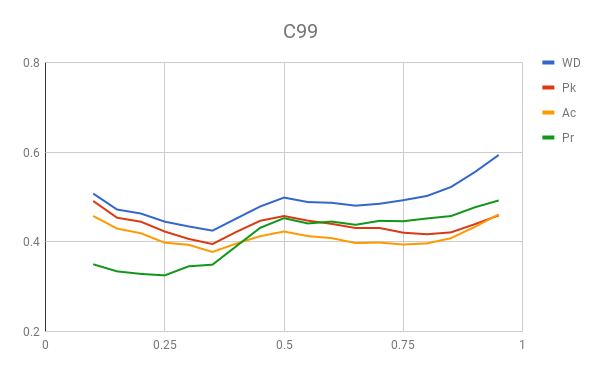
\includegraphics[width=.48\textwidth]{conteudo/capitulos/figs/graficos/analiseNSegRate-C99.png}
%	}
%	\subfigure{ \label{fig:influencia-segRate-mc}
	  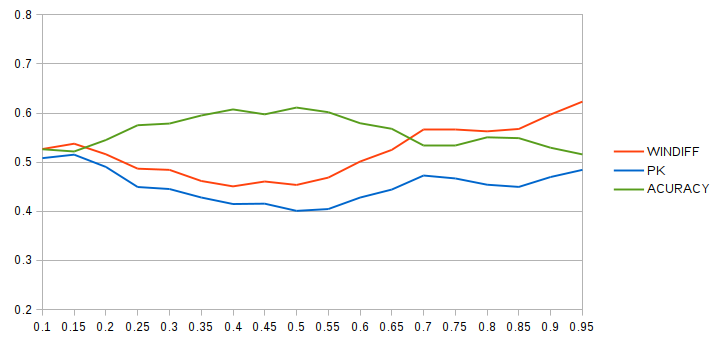
\includegraphics[width=.48\textwidth]{conteudo/capitulos/figs/graficos/analiseNSegRate-MinCut.png}
%	}
%	\subfigure{ \label{fig:influencia-segRate-bs}
	  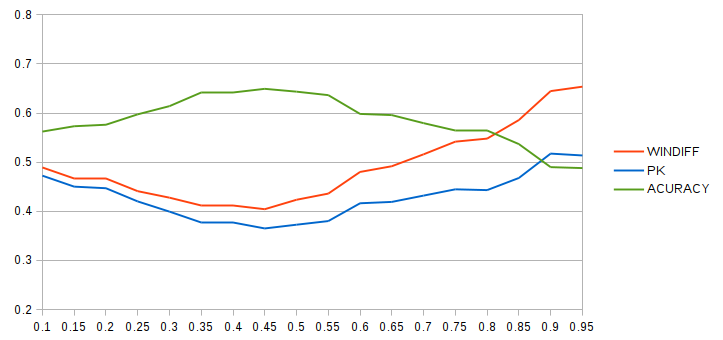
\includegraphics[width=.48\textwidth]{conteudo/capitulos/figs/graficos/analiseNSegRate-Bayes.png}
%	}
%	\subfigure{ \label{fig:influencia-segRate-ui}
	  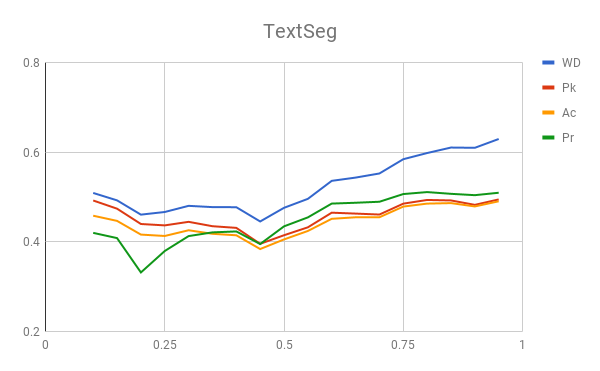
\includegraphics[width=.48\textwidth]{conteudo/capitulos/figs/graficos/analiseNSegRate-UISeg.png}
%	}
	\caption{Influência da taxa segmentos na eficiência dos algoritmos}
	\label{fig:influencia-SegRate}
\end{figure}




%%%%%%%%%%%%%%%%%%%%%%
% Análise da Coesão Léxica e eficiência da técnica do TT
%%%%%%%%%%%%%%%%%%%%%%

% --> Falar da coesão léxica peculiar das atas!!

A abordagem baseada em janelas deslisantes empregada no \textit{TextTiling} não permite a configuração direta da quantidade de segmentos extraídos, possibilitando o ajuste do tamanho do passo e comprimento da janela que influenciam seu comportamento nesse aspecto, os quais são analisados a seguir.
Uma vez que a coesão léxica é pressuposto de muitas abordagens em segmentação textual, fez-se uma análise desses documentos quanto a similaridade dos termos ao longo do texto. Verificou-se que a técnica de janelas deslizantes empregada pelo TextTiling encontra os vales que indicam transições entre segmentos. Contudo ao comparar esses vales com a segmentação de referência, nota-se que a maioria dos limites coincide ou estão próximos aos vales. Porém há casos onde a referência indica limites em trechos com alta coesão léxica e outros onde a queda da coesão, indicada por vales, não coincide com nenhum limite de referência.  

% Na Figura~\ref{fig:coesaolexicaTT}a linha horizontal representa a variação da coesão léxica ao longo de uma ata e as linha verticais azuis e vermelhas representam os limites entre segmentos atribuidos pela referência e pelo algoritmo respectivamente. 
Na Figura~\ref{fig:coesaolexicaTT} é apresentado a variação da coesão léxica ao longo de uma ata e a segmentação obtida pelo \textit{TextTiling} usando tamanho de janela igual a 50 e passo 9. 


  %--- ---
  \begin{figure}[!h]
	  \centering
	  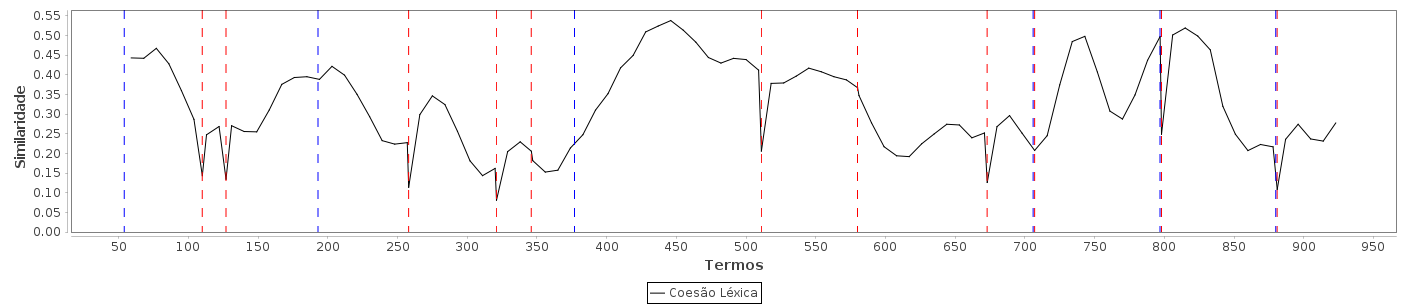
\includegraphics[width=\textwidth]{conteudo/capitulos/figs/coesaolexicaTT-50-9.png}
	  \caption{Variação da coesão léxica ao longo de uma ata junto a uma segmentação automática em contraste com uma segmentação de referência.
	  A linha horizontal representa a variação da coesão léxica e as linha verticais azuis e vermelhas representam os limites entre segmentos atribuídos pela referência e pelo algoritmo respectivamente. 
  }
	  \label{fig:coesaolexicaTT}
  \end{figure}









Em termos de performance, o modelo implementado no algoritmo \textit{BayesSeg} apresenta melhores resultados para as medidas $P_k$ e \textit{WindowDiff}, visto que essas são mais adequadas ao contexto analisado, este será empregado nos próximos experimentos. Contudo, dado a subjetividade da tarefa de segmentação textual, outros modelos podem ser utilizados satisfatoriamente dependendo do critério adotado. 


\begin{figure}[!ht] \centering     %%% not \center

%	\subfigure[a]{ 
		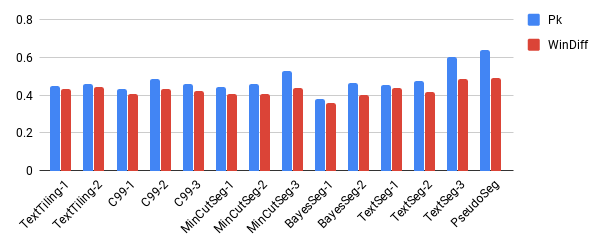
\includegraphics[width=.82\textwidth]{conteudo/capitulos/figs/graficos/resumo-wd-pk.png}	
		% \caption{wd-pk}
		\label{fig:resumo-wd-pka}
%	}
%	\subfigure[b]{ 
		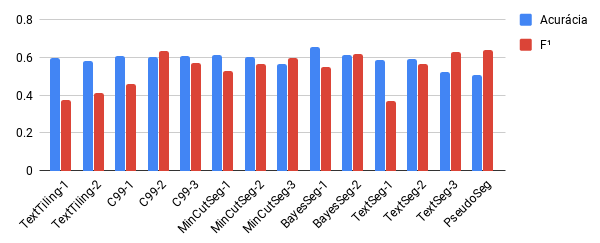
\includegraphics[width=.82\textwidth]{conteudo/capitulos/figs/graficos/resumo-tradicionais.png}	
		% \caption{tradicionais}
		\label{fig:resumo-tradicionaisa}
%	}
	\caption{Performance geral dos algoritmos de segmentação textual e as configurações que apresentam melhores resultados para cada medida de desempenho.}
	\label{fig:resumo-segmentadores}
\end{figure}



% TODO --> Comentar as WD e PK

Na Figura~\ref{fig:resumo-segmentadores} é apresentada a performance dos algoritmos.
% nas medidas tradicionais. 
Observa-se valores altos de $F^1$ para a segmentação por sentenças, pois é atribuído um limite a todo candidato a final de segmento, o que resulta no valor máximo para revocação. De maneira semelhante, o comportamento do \textit{TextTiling} gera menos segmentos em relação aos demais, e com isso tem-se valores menores de $F^1$, o que pode ser alterado pela configuração do algoritmo com passos mais curtos, ou ainda, sobre-escrevendo a função que calcula os \textit{depth scores} para reconhecer vales menos profundos.



% De maneira geral, os métodos probabilísticos apresentam desempenho próximo 



Após a análise dos métodos, selecionou-se o algoritmo \textit{BayesSeg} para a tarefa de segmentação textual nesse trabalho. 
A escolha justifica-se por este algoritmo apresentar melhores resultados para as medidas $P_k$ e \textit{WindowDiff} visto a subjetividade da tarefa e a aderência dessas medias à acurácia e precisão. Mais análises quanto à segmentação textual e desempenho do \textit{BayesSeg} serão abordadas no Capítulo~\ref{cap-extratores}. Em que realizou-se então uma experimento a fim de avaliar subjetivamente o segmentador escolhido em conjunto com extratores de tópicos.




  % Após a identificação dos segmentos, o algoritmo retorna uma lista com fragmentos do texto original. Cada segmento é incorporado à estrutura de dados interna como subdocumentos com um tema relativamente independente. Em seguida, esses subdocumentos serão analisados pelo extrator de tópicos para identificação de descritores e agrupamento.



\section{Considerações Finais}



Nessa seção os algoritmos de segmentação textual foram avaliados objetivamente. 
Inicialmente, criou-se um conjunto com segmentações manuais usados para gerar uma segmentação de referência, sob a qual os resultados dos algoritmos foram comparados. O produto  desse processo também foi acrescido de rótulos e descrições sobre o assunto de cada segmento.
Embora a concordância sobre a segmentação entre anotadores tenha se mostrado abaixo do esperado, obteve-se, \textit{corpus} anotado que ajuda a entender a coleção de atas original em termos de transição de assuntos entre segmentos e seus conteúdos.
% em termos da distribuição de tópicos. 
Contudo, mais experimentos são necessários para criação de uma segmentação de referência mais robusta, a qual pode ser obtida com maior número de anotadores, e aperfeiçoamento do processo de anotação. Após esses primeiros resultados, melhorias na ferramenta para segmentação manual e aplicação de um treinamento adequado dos participantes podem ser desenvolvidos com base nessa primeira experiência.
% , bem como avaliação de técnicas que se valem de conhecimento externo como \textit{thesaurus} (dicionários) e \textit{clue words} (palavras-pista).

De maneira geral, os dados apontam que há pouca diferença de performance entre os algoritmos de segmentação textual. Contudo, o \textit{BayesSeg} mostrou-se superior aos demais considerando-se a similaridades entre seus resultados e a segmentação de referência, as quais foram mensuradas pelas medidas \textit{WindowDiff} e $P_k$.  
Uma análise subjetiva do segmentador escolhido é apresentada na Seção~\ref{cap-extratores}, em que observa-se resultados satisfatórios a repeito da qualidade dos segmentos obtidos. 

O \textit{corpus} criado a partir da coleção original de documentos foi disponibilizados para trabalhos futuros voltados a esse domínio bem como o \textit{software} para segmentação manual e rotulação de documentos. 


% por meio de um corpus gerado a partir de






























